\subsection{Upper limits on SMS models}
%
For each mass-pair ($m_{\st},m_{LSP}$) in a given model described in Section~\ref{sec:signal}, 
the upper limit is calculated as described in Section~\ref{sec:cls} using the likelihood 
constructed in Section~\ref{sec:likelihood} by considering the relevant categories 
listed in Table~\ref{tab:simplified-models}.


\subsubsection{Upper limits on T2cc}
The color scale in Figure~\ref{fig:upperLimits-t2cc} shows the observed upper 
limit at 95\% confidence level for each sparticle mass-pair bin in the SMS 
model where a stop particle decays to a charm quark and a neutralino (\texttt{T2cc}). 
The mass-pair bins left of the thick black curve have a calculated cross 
section upper limit below the theoretical production cross section, 
i.e. $\frac{\sigma_{\texttt{obs. upper limit}}}{\sigma_{\texttt{theory}}} < 1$, and
are therefore excluded. The thinner black lines represent exclusion regions obtained by
comparing the calculated upper limit with the theoretical cross section shifted up down 
and by its theoretical uncertainty i.e. 
$\frac{\sigma_{\texttt{obs. upper limit}}}{\sigma_{\texttt{theory} \pm \texttt{uncertainty}}} < 1$.
The dashed purple lines indicate the median (thick line) $\pm 1 \sigma$ 
(thin lines) expected exclusion regions. The $\pm 1 \sigma$ expected exclusion 
regions are not obtained by varying the theoretical cross section but rather 
by comparing the calculated expected upper limit $\pm 1 \sigma$ uncertainty
with the nominal cross section. The observed upper limit curve lies within
$+1 \sigma$ expected curve. For comparison, Figure~\ref{fig:atlas} shows similar
exclusion limits obtained by the ATLAS collaboration~\cite{Aad:2008zzm} for the same 
model. 

\begin{figure}[h!]
  \begin{center}
  \subfigure[\label{fig:upperLimits-t2cc}]{
    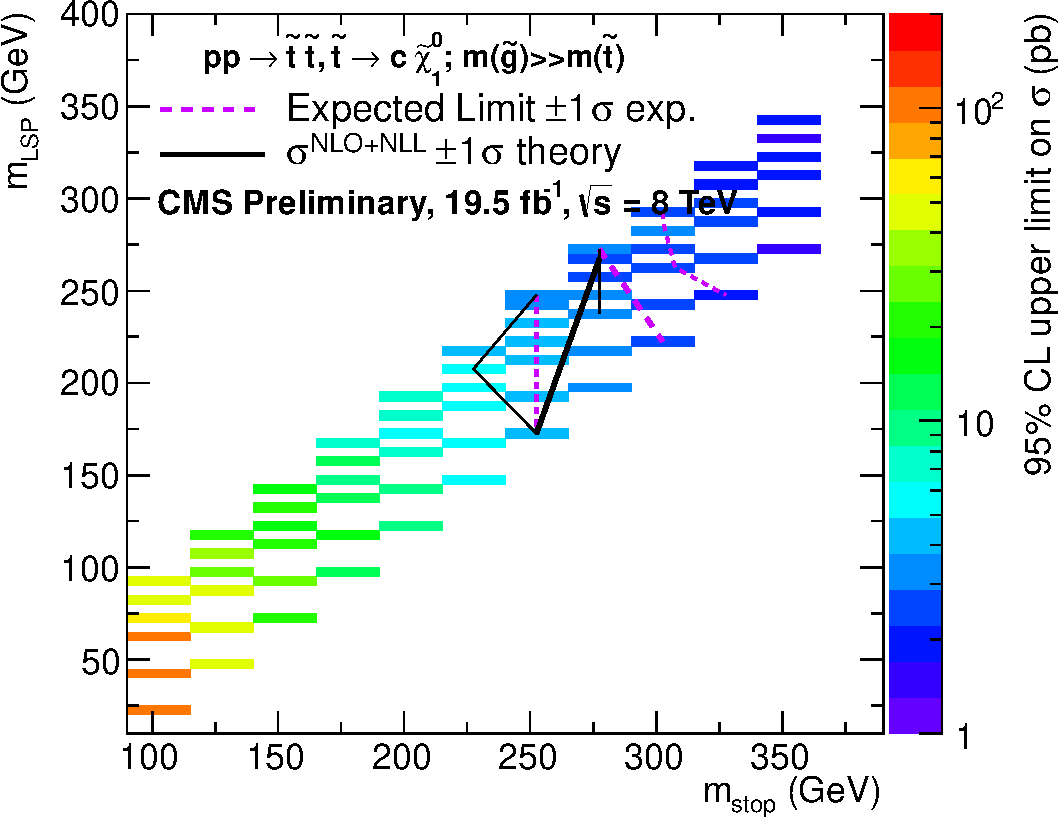
\includegraphics[width=0.45\textwidth,clip=true]{figures/limits/merged/T2cc/v2/CLs_frequentist_T2cc_2012pf_0b_le3j_0b_ge4j_1b_ge4j_xsLimit}
    }   
  \subfigure[\label{fig:atlas}]{     
    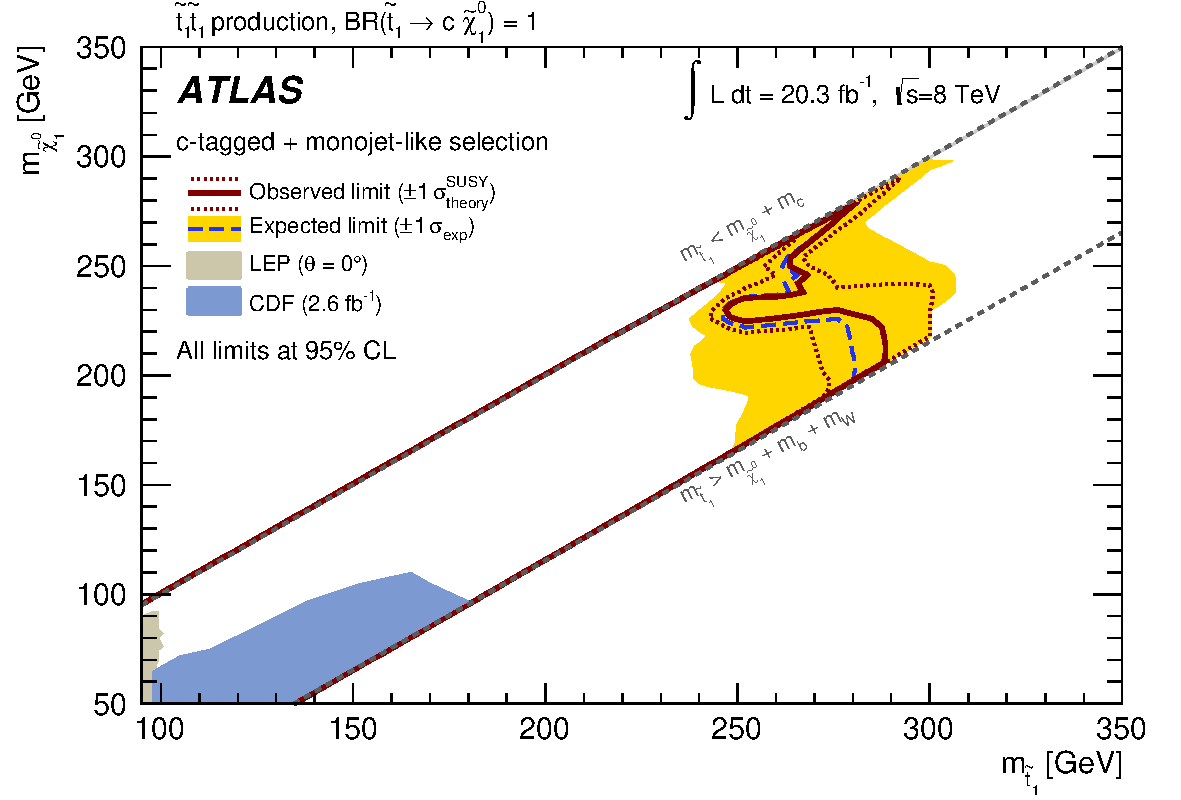
\includegraphics[width=0.45\textwidth,clip=true]{figures/limits/merged/T2cc/v2/atlas}
    }   
    \caption{(a) The expected and observed upper limits at 95\% C.L. on the production cross section 
    for the for the model \texttt{T2cc} obtained in this analysis. See text for details on each curve.
    (b) Exclusion region in the same model obtained by the ATLAS collaboration, from Ref.~\cite{Aad:2014nra}
    Mass pairs left (and below) of the observed limit are excluded at the 95\% C.L.}
  \end{center}
\end{figure}

\subsubsection{Upper limits on T2tt}

The color scale in Figure~\ref{fig:upperLimits-t2tt} shows the observed upper 
limit at 95\% confidence level for each sparticle mass-pair bin in the SMS 
model where a stop particle decays to a top quark and a neutralino (\texttt{T2tt}). 
The definitions of the excluded regions remain the same as \texttt{T2cc}.
The observed upper limit disagrees with the expected by more than $2\sigma$.

\begin{figure}[h!]
  \begin{center}
      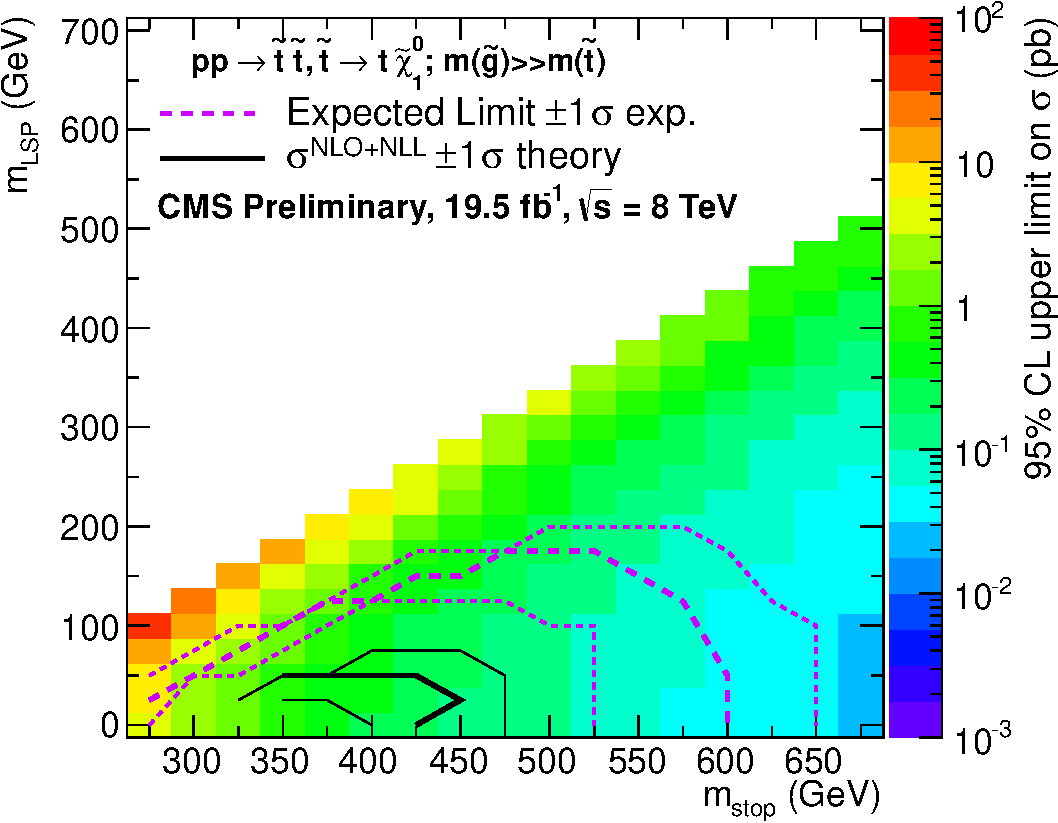
\includegraphics[width=0.70\textwidth,clip=true,]{figures/limits/merged/T2tt/v6/CLs_frequentist_T2tt_2012pf_1b_ge4j_2b_ge4j_xsLimit}
    \caption{\label{fig:upperLimits-t2tt}Expected and observed upper limits on the production cross section 
    for the models \texttt{T2tt}. Mass pairs left (and below) of the observed limit are excluded at the 95\% C.L.}
  \end{center}
\end{figure}

\FloatBarrier

It is instructive to re-examine the \scalht bins which show the highest excesses 
when considering a SM-only hypotheses. To this intent, Figure~\ref{fig:sigVsCat} of 
Section~\ref{sec:results} is re-plotted in Figure~\ref{fig:sigVsCat2} to 
isolate the categories used in interpreting \texttt{T2tt}. In the \njethigh 
and $\nb = 2$ category, \scalht bins $575-675$ and $675-775\GeV$ show excesses of 
$\sim\!\!2.5\sigma$ and $\sim\!\!1.5\sigma$ respectively. In the \njethigh and 
$\nb = 1$ category, the lowest two \scalht bins are $\sim\!\!1.5\sigma$ 
from expectation. More generally, the categories used to interpret \texttt{T2tt} can be
characterized by mild excesses in the lowest \scalht bins and with
a more pronounced excess in \scalht = $575~\GeV-675~\GeV$ in \njethigh 
and $\nb = 2$ category. 
\begin{figure}[h!]
  \begin{center}
      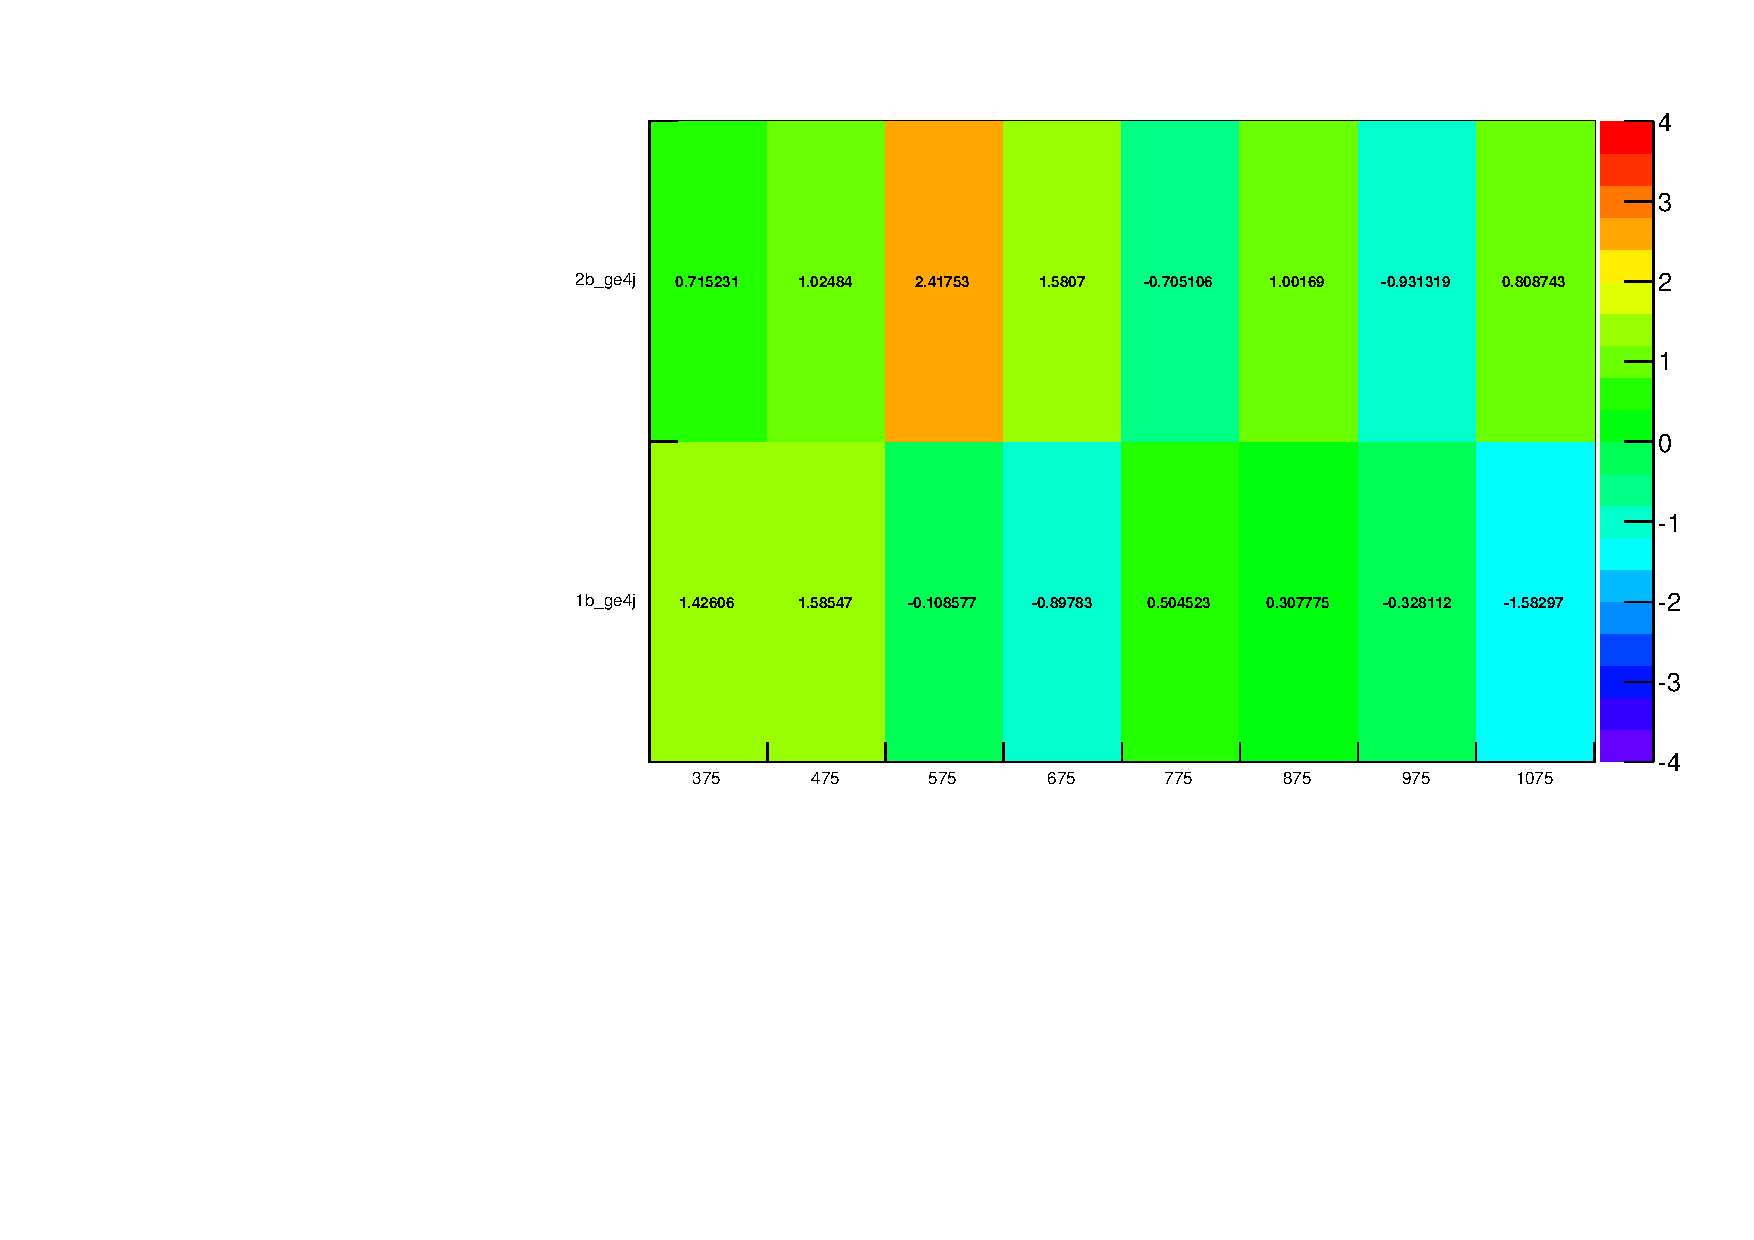
\includegraphics[width=0.75\textwidth, trim=0 0 0 30, clip=true]{figures/fit/v22/significances_catVsHt_2}
    \caption{Pulls in categories used in T2cc interpretation.\label{fig:sigVsCat2}}
  \end{center}
\end{figure}
%\FloatBarrier
The discrepancy in the observed and expected 
limit is better understood with a closer study of the mass-pair
bin ($m_{\st} = 400\GeV$, $m_{\text{LSP}} = 0\GeV$), which is 
expected to be excluded but it is not by the observed data. 
It is useful to gauge the signal significance, defined here as the signal 
yield divided by $\sqrt{b+(0.1b)^2}$ where $b$ is the SM expectation (background) 
as determined by a simultaneous fit to all control data samples under the SM background 
hypothesis. Figure~\ref{fig:t2tt-sig-400_100} plots the signal significance in bins of 
\scalht and shows that most of the significance is expected in the 
lower \scalht bins in both categories. Furthermore, 
figure~\ref{fig:t2tt-best-fit-400_100} shows the \scalht-binned 
observed data yields and expectations for the hadronic sample, as determined 
by a simultaneous fit to all data samples under a signal+background 
hypothesis. The signal under consideration remains $m_{\st} = 400\GeV$ and 
$m_{\text{LSP}} = 100\GeV$. The fit is performed simultaneously across 
both event categories. The plots give the indication that while the excesses 
in the low \scalht bins are mild, they are enough to accommodate a signal-like
excess.\\
\indent Finally, a profile likelihood ratio scan is performed 
to visualize the best fit and upper limit at 95\% C.L. values 
on the signal strength. The result is shown in Figure~\ref{fig:t2tt-int-400_100}.
%A similar disagreement between observed and expected
%exclusions was observed in the latest published 

%The descripency the observed and expected limit is further investigated 
%by a closer study of two bins in $(m_{\st},m_{\text{LSP}})$. 
%The first one, $m_{\st} = 400\GeV$ and $m_{\text{LSP}} = 0\GeV$ 
%is excluded by the observed data. It is useful to gauge the signal 
%signifcance, defined here as the signal yield divided by $\sqrt{b+(.1b)^2}$ 
%where $b$ is the SM expectation as determined by a simultaneous 
%fit to all under under the SM background hypothesis. 
%Figure~\ref{fig:t2tt-sig-400} plots the signal significance in bins of 
%\scalht and shows that most of the significance is expected in the 
%lowest \scalht bins in both categories. Furthermore, 
%figure~\ref{fig:t2tt-best-fit-400} shows the \scalht-binned 
%observed data yields and expectations for the hadronic sample, as determined 
%by a simultaneous fit to all data samples under a signal+background 
%hypothesis. The signal under consideration remains $m_{\st} = 400\GeV$ and 
%$m_{\text{LSP}} = 0\GeV$. The fit is performed simultaneously across 
%both event categories. Finally, a profile likelihood ratio scan is performed 
%as a function of signal strength to vizualize the signal strength value 
%best fitting the data and the upper limit on that signal strength
%at 95\% confidence level. 
%To summarize, the excesses are mild enough and the 
%prodcution cross secton for the signal bin $m_{\st} = 400\GeV$ 
%and $m_{\text{LSP}} = 0\GeV$, 
%
%As the production cross section of pair produced stops decreases with
%increasing stop mass, the overall signal significance drops. Furthermore
%the shape of the  

%\begin{table}[h!]
%  \caption{The first two columns specify the model and its
%    production and decay. The next column specifies the event
%    categories (in terms of \njet and
%    \nb) considered for each interpretation. The last 
%    two columns indicate the search sensitivity for each model,
%    where $m_{\st(\sGlu)}^{\textrm{best}}$ and
%    $m_{\textrm{LSP}}^{\textrm{best}}$ represent the largest mass 
%    beyond which no limit can be set for squarks/gluinos and the LSP,
%    respectively. The exclusion range for $m_{\st(\sGlu)}$ is bounded
%    from below by the kinematic region considered for each model, as
%    defined in the text. The quoted estimates are determined 
%    conservatively from the observed exclusion based on the
%    theoretical production cross section minus $1\sigma$
%    uncertainty. 
%    %For model \texttt{T2tt}, the search is at the threshold of
%    %sensitivity for the considered ($m_{\stua},m_{\rm LSP}$) parameter
%    %space, as discussed in the text. 
%  }  
%  \label{tab:sms}
%  \centering
%  \footnotesize
%  \begin{tabular}{ llcccc }
%    \hline
%    Model
%    & Production/decay
%    & Event categories
%    & Limit plot
%%    & $m_{\st(\sGlu)}^{\textrm{best}}$~(GeV) 
%%    & $m_{\textrm{LSP}}^{\textrm{best}}$~(GeV) 
%    \\ [0.5ex]
%    \hline
%    \texttt{T2cc}
%    &
%    $\textrm{pp}\,\rightarrow\,\sTop\sTop\,\rightarrow\,\textrm{c}\chiz\bar{\textrm{c}}\chiz$
%    & ($\le3$,0), ($\ge4$,0), ($\ge4$,1)
%    & \ref{fig:upperLimits-t2cc}
%%    & 250
%%    & 250
%     \\
%    \texttt{T2tt} 
%    & 
%    $\textrm{pp}\,\rightarrow\,\sTop\sTop\,\rightarrow\,\textrm{t}\chiz\bar{\textrm{t}}\chiz$
%    & ($\geq4$,1),($\geq4$,2)
%    & \ref{fig:upperLimits-t2tt}
%%    & 400 
%%    & 25
%    \\ 
%    \hline
%  \end{tabular}
%\end{table}

%\fixme{TEXT REFLECTS USUAL PRESENTATION OF LIMIT PLOTS - ALL RELEVANT
%  INFORMATION IN SHOWN IN REFERENCED FIGURES FOR T2CC - TO BE UPDATED.}
%Figures~\ref{fig:limits-t2cc-exp} and \ref{fig:limits-t2cc-obs} show
%the upper limit on the cross section at 95\% CL as a function of
%$m_{\st}$ or $m_{\gl}$ and $m_{\rm LSP}$ for various simplified
%models. The point-to-point fluctuations are due to the finite number
%of pseudo-experiments used to determine the observed upper limit. The
%solid thick black line indicates the observed exclusion region
%assuming NLO+NLL~\cite{Beenakker:1996ch, susy-nlo-nll} SUSY cross
%section for squark pair production in the limit of very massive
%gluinos (or vice versa). The thin black lines represent the observed
%excluded region when varying the cross section by its theoretical
%uncertainty. The dashed purple lines indicate the median (thick line)
%$\pm 1 \sigma$ (thin lines) expected exclusion regions.
%
%%Figure~\ref{fig:t2cc-1d} shows the observed upper limit at 95\% CL on
%%the production cross section as a function of the top squark mass
%%($m_{\sTop}$) for the model \texttt{T2cc} when considering two
%%different \sTop-\chiz mass splittings of $\Delta m = 10\gev$ (left)
%%and $\Delta m = 80\gev$ (right). The observed upper limit (95\% CL) on
%%the production cross section is shown as a function of $m_{\sTop}$
%%(solid line), along with the expected upper limit and
%%$\mathbf{\pm2}\sigma$ {\bf experimental uncertainties} (long-dashed
%%line with shaded band), and the NLO+NLL top squark pair-production
%%cross section and theoretical uncertainties (dotted line with shaded
%%band).
%
%Figure~\ref{fig:t2cc-best-fit} shows the \scalht-binned observed data
%yields and expectations for the hadronic sample, as determined by a
%simultaneous fit to all data samples under the signal+background
%hypothesis. The observed event yields in data (black dots), the SM
%expectations (dark blue) and the sum of the SM backgrounds and signal
%expectation (pink) are shown. The signal expectations are for the best
%fit model \texttt{T2cc} with $m_{\st} = 250\GeV$ and $m_{\text{LSP}} =
%230\GeV$. Three event categories are considered by the fit: (Top)
%\njetlow and $\nb = 0$, (Middle) \njethigh and $\nb = 0$, (Bottom)
%\njethigh and $\nb = 1$. The fit is performed (Left) for each
%individual event category or (Right) simultaneously across all three
%event categories.
%
%\begin{figure}[h!]
%  \begin{center}
%    \subfigure[$+1\sigma$ experimental, relative]{
%      \includegraphics[width=0.45\textwidth,page=3,trim=40 50 20 70,clip=true]{figures/limits/v0/exp/CLs_frequentist_T2cc_2012dev_0b_le3j_0b_ge4j_1b_ge4j_xsLimit_relative}
%    } \quad
%    \subfigure[$+1\sigma$ experimental, excluded points]{
%      \includegraphics[width=0.45\textwidth,page=3,trim=40 50 20 70,clip=true]{figures/limits/v0/exp/CLs_frequentist_T2cc_2012dev_0b_le3j_0b_ge4j_1b_ge4j_xsLimit_simpleExcl}
%    } \\
%    \subfigure[Nominal, relative]{
%      \includegraphics[width=0.45\textwidth,page=1,trim=40 50 20 70,clip=true]{figures/limits/v0/exp/CLs_frequentist_T2cc_2012dev_0b_le3j_0b_ge4j_1b_ge4j_xsLimit_relative}
%    } \quad 
%    \subfigure[Nominal, excluded points]{
%      \includegraphics[width=0.45\textwidth,page=1,trim=40 50 20 70,clip=true]{figures/limits/v0/exp/CLs_frequentist_T2cc_2012dev_0b_le3j_0b_ge4j_1b_ge4j_xsLimit_simpleExcl}
%    } \\
%    \subfigure[$-1\sigma$ experimental, relative]{
%      \includegraphics[width=0.45\textwidth,page=2,trim=40 50 20 70,clip=true]{figures/limits/v0/exp/CLs_frequentist_T2cc_2012dev_0b_le3j_0b_ge4j_1b_ge4j_xsLimit_relative}
%    } \quad 
%    \subfigure[$-1\sigma$ experimental, excluded points]{
%      \includegraphics[width=0.45\textwidth,page=2,trim=40 50 20 70,clip=true]{figures/limits/v0/exp/CLs_frequentist_T2cc_2012dev_0b_le3j_0b_ge4j_1b_ge4j_xsLimit_simpleExcl}
%    } \\
%    \caption{\label{fig:limits-t2cc-exp} \fixme{TEMPORARY PLACE
%        HOLDERS FOR THE FINAL LIMIT PLOT. HOWEVER, ALL RELEVANT
%        INFORMATION IS CONTAINED HERE.} Expected limits for the model 
%      \texttt{T2cc}. In the left column, the plots show the upper
%      limit on the production cross section relative to the
%      theoretical value. In the right column, the plots show the mass
%      points that are excluded (marked red). In all plots, the yellow
%      line should be ignored. The expected limits are shown in the
%      middle row, with limits corresponding to the $+1\sigma$ and
%      $+1\sigma$ variations in the experimental uncertainties shown
%      top and bottom, respectively. }
%  \end{center}
%\end{figure}
%
%\begin{figure*}[t!]
%  \begin{center}
%     \subfigure[\njethigh, $\nb = 1$, simultaneous fit]{
%      \includegraphics[width=0.45\textwidth,page=13]{figures/fit/v22/stackedSig/400_0/bestFit_2012pf_RQcdZero_fZinvAll_1b_ge4j-1p_2b_ge4j-1_sel1b_ge4j_smOnly.pdf}
%    } 
%    \subfigure[\njethigh, $\nb = 2$, simultaneous fit]{
%      \includegraphics[width=0.45\textwidth,page=9]{figures/fit/v22/stackedSig/400_0/bestFit_2012pf_RQcdZero_fZinvAll_1b_ge4j-1p_2b_ge4j-1_sel2b_ge4j_smOnly.pdf}
%    } \\
%    \caption{\label{fig:t2tt-sig-400} The \scalht-binned 
%      signal significance defined as the signal yield 
%      divided by the $\sqrt{b+(.1b)^2}$ where $b$ is the
%      SM expectation obtained by a fit to all 
%      control data samples under the SM-only background 
%      hypothesis for the two categories (a) \njethigh, $\nb = 1$ and (b) 
%      \njethigh, $\nb = 2$ simultaneously. 
%      The signal model is \texttt{T2tt} with 
%      $m_{\st} = 400\GeV$ and $m_{\text{LSP}} = 0\GeV$.} 
%  \end{center}
%\end{figure*}
%

%\begin{figure*}[t!]
%  \begin{center}
%    \subfigure[\njethigh, $\nb = 1$, simultaneous fit]{
%      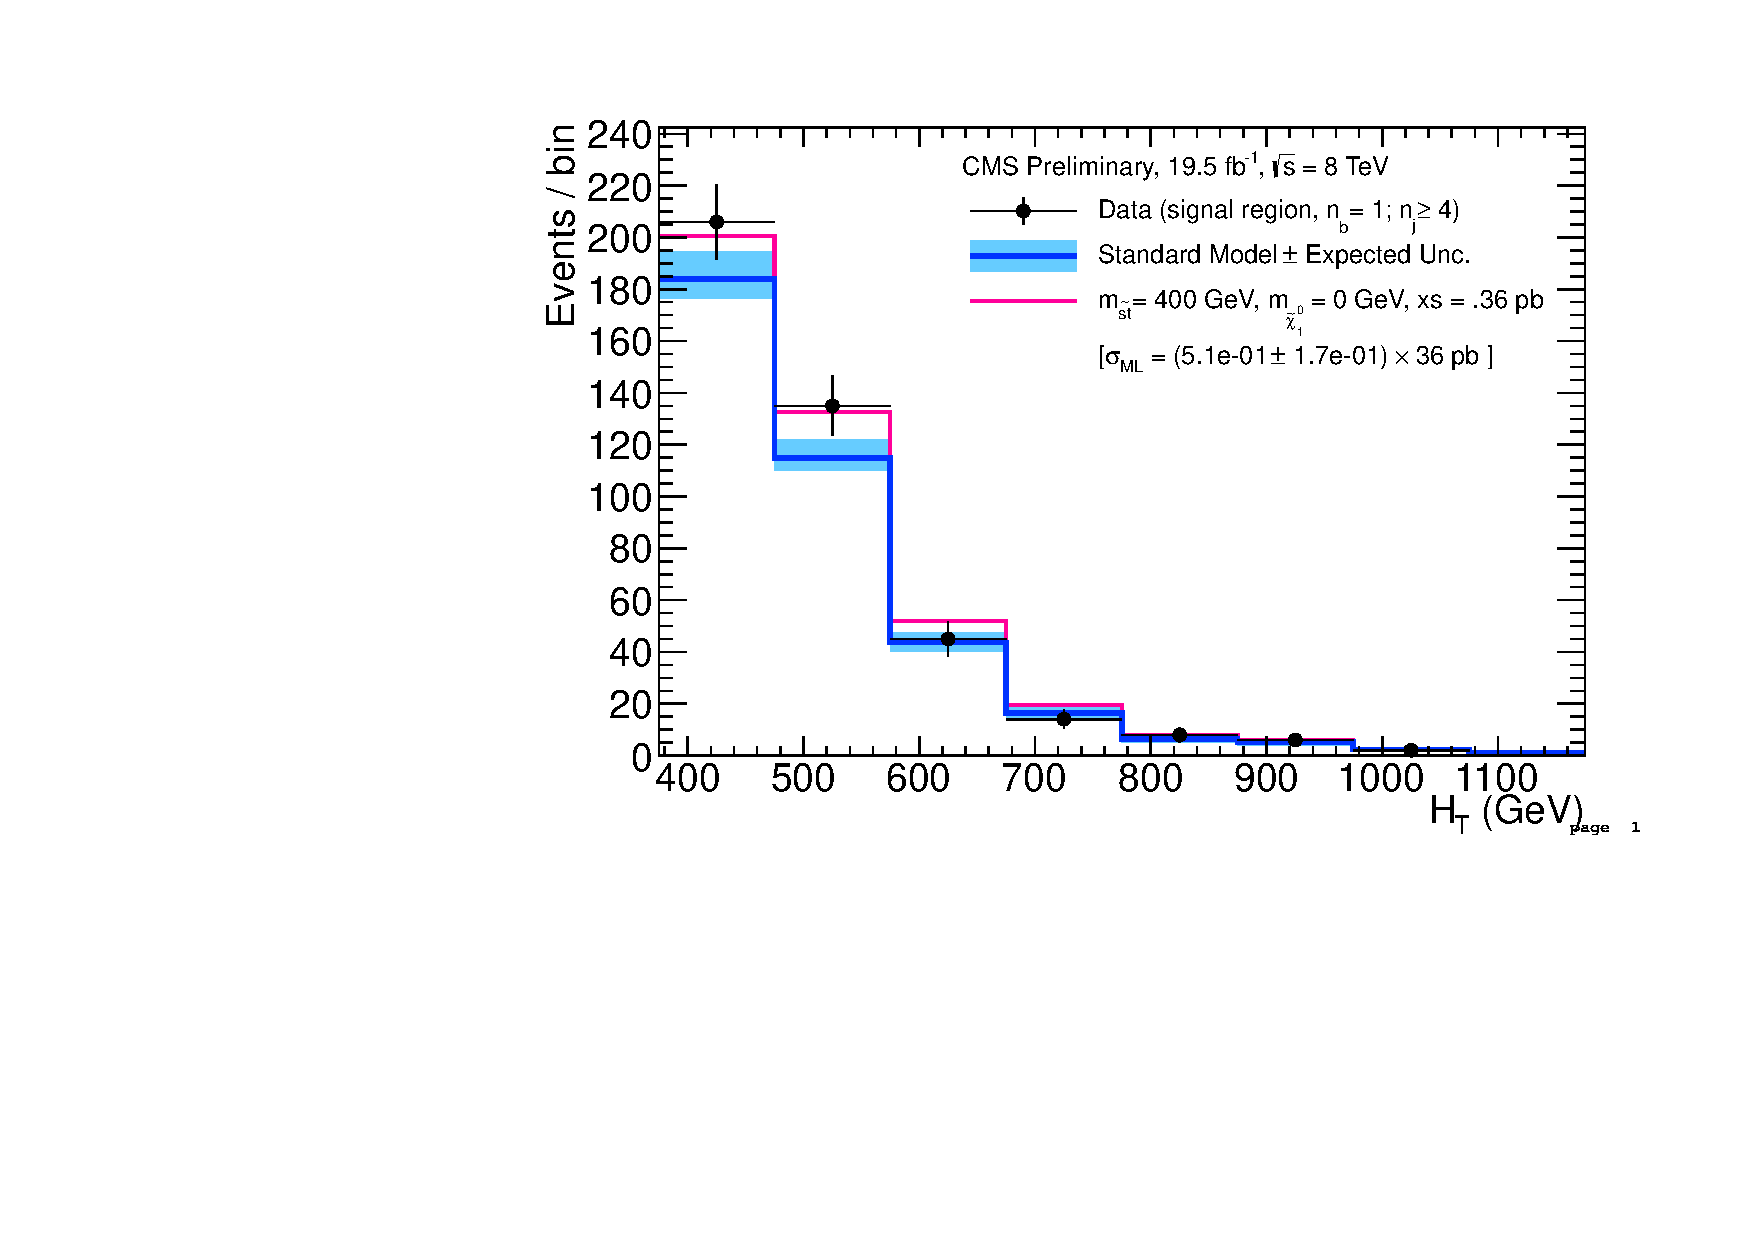
\includegraphics[width=0.45\textwidth]{figures/fit/v22/wSignal/400_0/bestFit_2012pf_RQcdZero_fZinvAll_1b_ge4j-1hp_2b_ge4j-1h_signal_sel1b_ge4j}
%    } 
%    \subfigure[\njethigh, $\nb = 2$, simultaneous fit]{
%      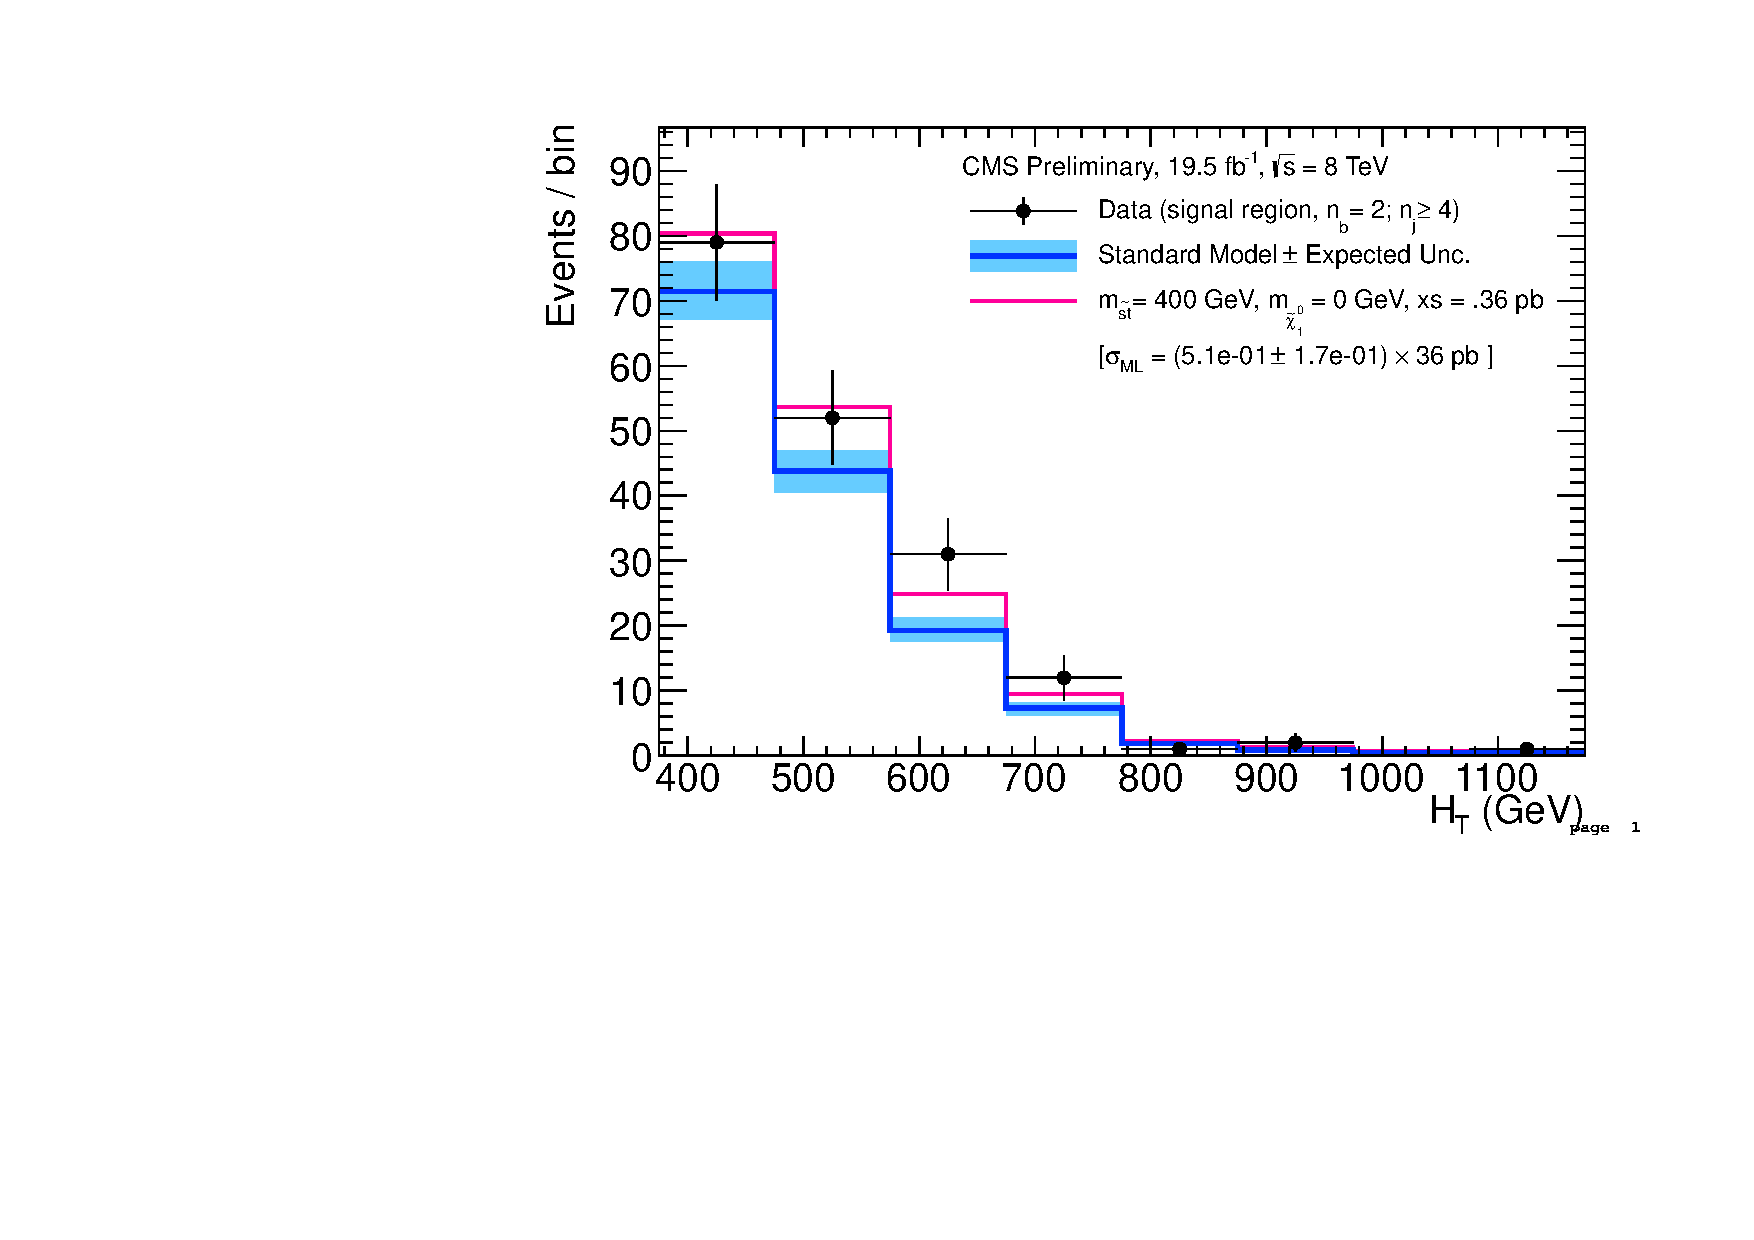
\includegraphics[width=0.45\textwidth]{figures/fit/v22/wSignal/400_0/bestFit_2012pf_RQcdZero_fZinvAll_1b_ge4j-1hp_2b_ge4j-1h_signal_sel2b_ge4j}
%    } \\
%    \caption{\label{fig:t2tt-best-fit-400}The comparison of
%      the \scalht-binned observed data yields and expectations for the
%      hadronic sample, as determined by a simultaneous fit to all data
%      samples under the signal plus SM background hypothesis. The
%      observed event yields in data (black dots), the SM expectations
%      (dark blue solid line), and the signal expectations (pink solid
%      line), as determined by the simultaneous fit, for the 
%      signal model \texttt{T2tt} with $m_{\st} = 400\GeV$ and
%      $m_{\text{LSP}} = 0\GeV$. Two event categories are
%      considered: (a) \njethigh and $\nb = 1$, (b) \njethigh and
%      $\nb = 2$.}
%  \end{center}
%\end{figure*}
%\begin{figure*}[t!]
%  \begin{center}
%    \subfigure[profile likelihood ratio, simultaneous fit]{
%      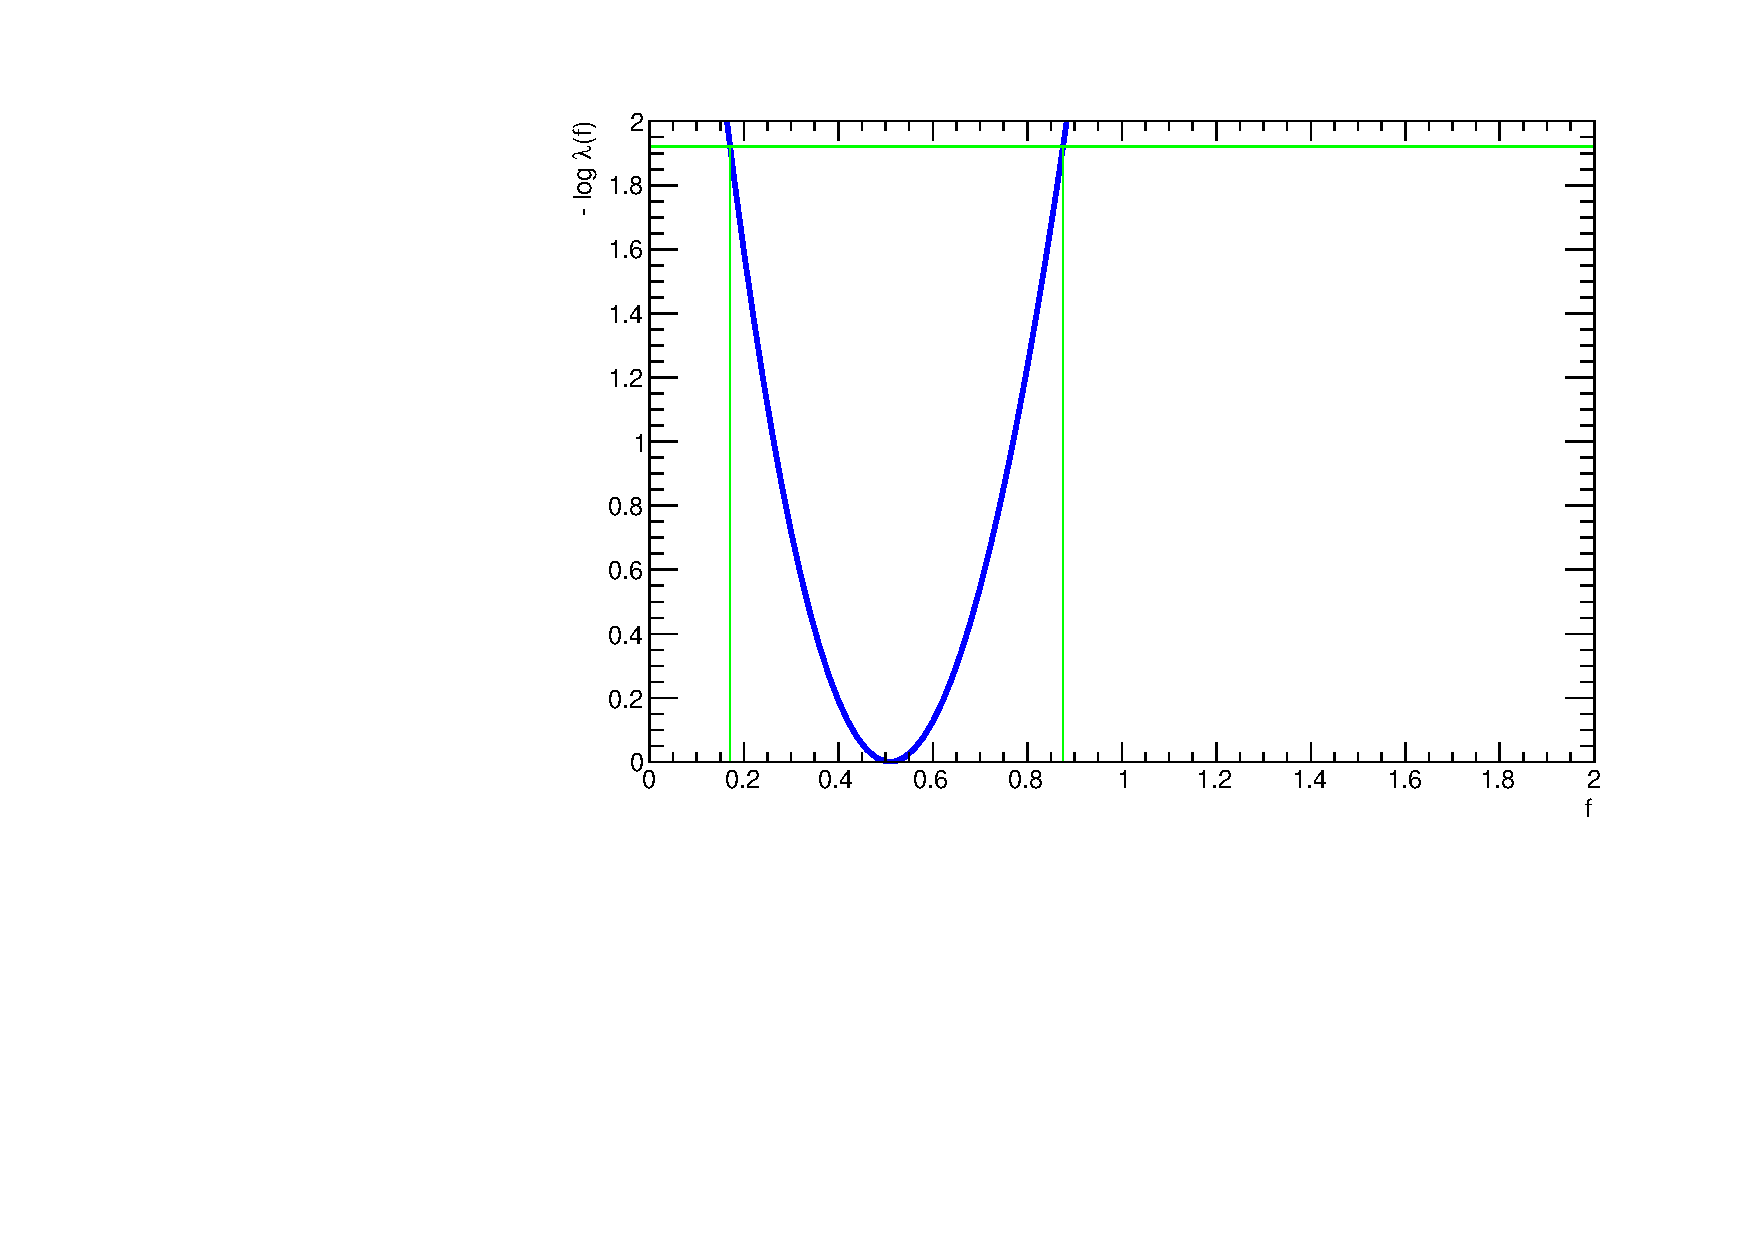
\includegraphics[width=0.45\textwidth]{figures/fit/v22/wSignal/400_0/intervalPlot_2012pf_RQcdZero_fZinvAll_1b_ge4j-1hp_2b_ge4j-1h_signal_95}
%    } \\
%    \caption{\label{fig:t2cc-int-400}The profile likelihood ratio 
%      (defined in sec.~\ref{sec:cls}) as a function of the signal strength.
%      The likelihood considers all data samples under the signal plus SM 
%      background hypothesis for the signal model \texttt{T2tt} with 
%      $m_{\st} = 400\GeV$ and $m_{\text{LSP}} = 0\GeV$.
%      The minimum defines the signal strength estimate which maximizes the
%      likelihood and the green vertical line on the right of the minimum 
%      indicates the upper-limit at 95\% confidence level.}
%  \end{center}
%\end{figure*}
%
%\clearpage
\begin{figure*}[h!]
  \begin{center}
     \subfigure[\njethigh, $\nb = 1$, simultaneous fit]{
      \includegraphics[width=0.45\textwidth,page=13]{figures/fit/v22/stackedSig/400_100/bestFit_2012pf_RQcdZero_fZinvAll_1b_ge4j-1p_2b_ge4j-1_sel1b_ge4j_smOnly.pdf}
    } 
    \subfigure[\njethigh, $\nb = 2$, simultaneous fit]{
      \includegraphics[width=0.45\textwidth,page=9]{figures/fit/v22/stackedSig/400_100/bestFit_2012pf_RQcdZero_fZinvAll_1b_ge4j-1p_2b_ge4j-1_sel2b_ge4j_smOnly.pdf}
    } \\
    \caption{\label{fig:t2tt-sig-400_100} The \scalht-binned 
      signal significance defined as the signal yield 
      divided by the $\sqrt{b+(.1b)^2}$ where $b$ is the
      SM expectation obtained by a fit to all 
      control data samples under the SM-only background 
      hypothesis for the two categories (a) \njethigh, $\nb = 1$ and (b) 
      \njethigh, $\nb = 2$ simultaneously. 
      The signal model is \texttt{T2tt} with 
      $m_{\st} = 400\GeV$ and $m_{\text{LSP}} = 100\GeV$.} 
  \end{center}
\end{figure*}

\begin{figure*}[h!]
  \begin{center}
    \subfigure[\njethigh, $\nb = 1$, simultaneous fit]{
      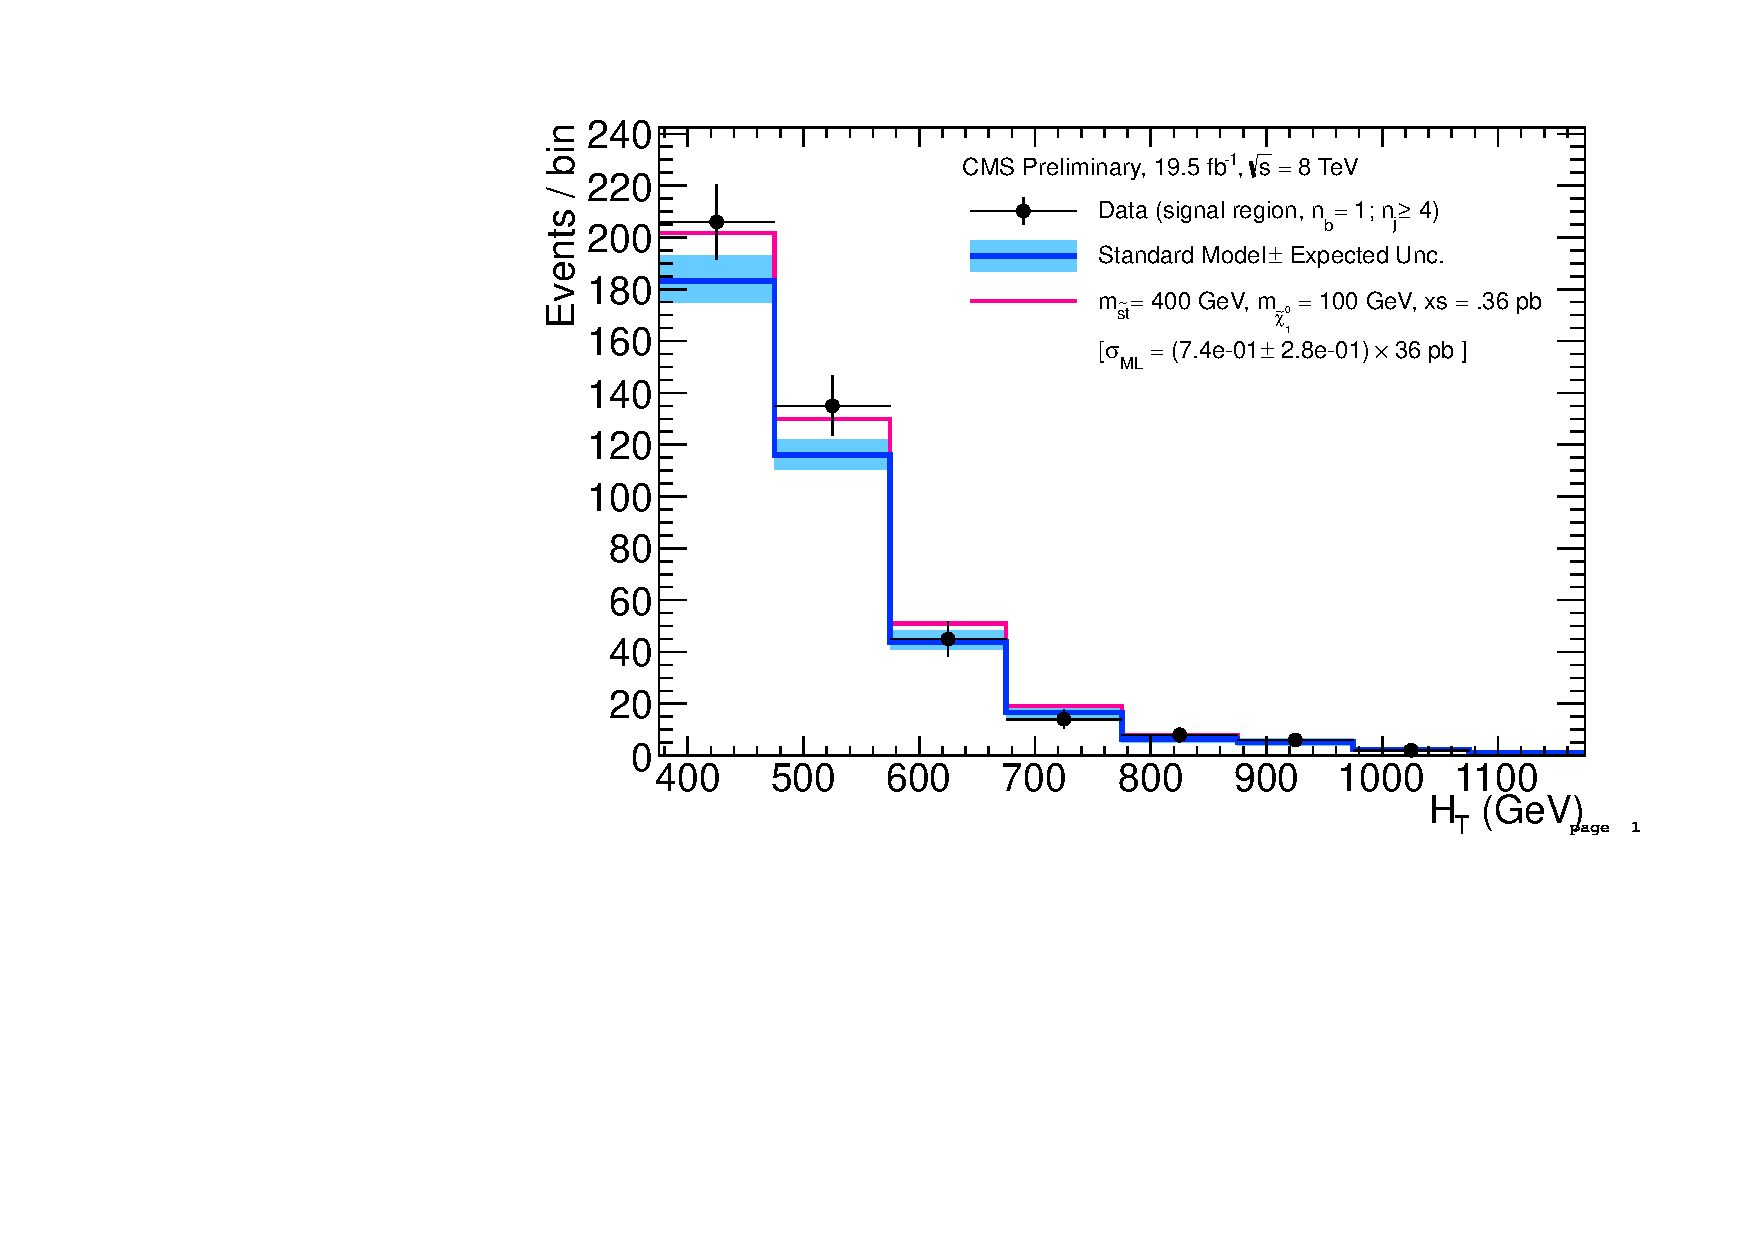
\includegraphics[width=0.45\textwidth]{figures/fit/v22/wSignal/400_100/bestFit_2012pf_RQcdZero_fZinvAll_1b_ge4j-1hp_2b_ge4j-1h_signal_sel1b_ge4j}
    } 
    \subfigure[\njethigh, $\nb = 2$, simultaneous fit]{
      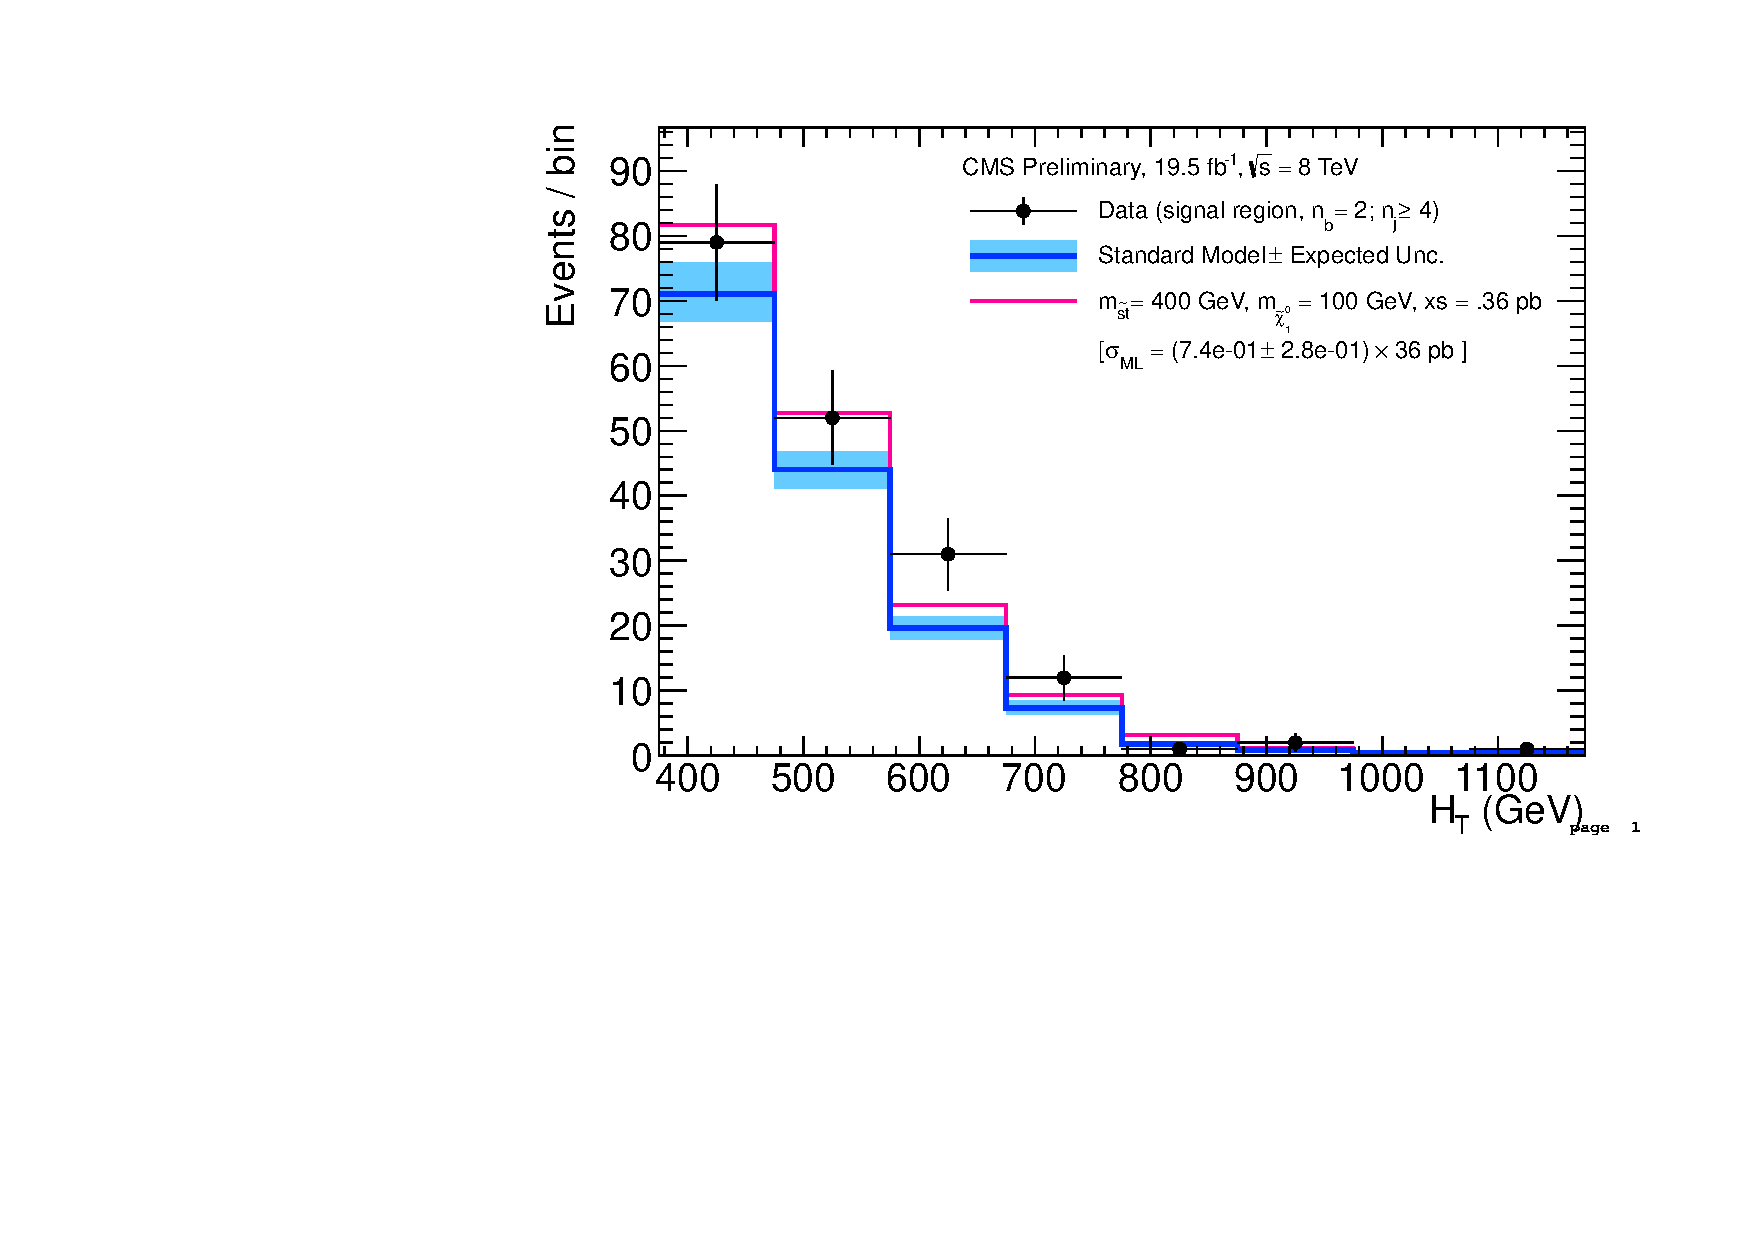
\includegraphics[width=0.45\textwidth]{figures/fit/v22/wSignal/400_100/bestFit_2012pf_RQcdZero_fZinvAll_1b_ge4j-1hp_2b_ge4j-1h_signal_sel2b_ge4j}
    } \\
    \caption{\label{fig:t2tt-best-fit-400_100}The comparison of
      the \scalht-binned observed data yields and expectations for the
      hadronic sample, as determined by a simultaneous fit to all data
      samples under the signal plus SM background hypothesis. The
      observed event yields in data (black dots), the SM expectations
      (dark blue solid line), and the signal expectations (pink solid
      line), as determined by the simultaneous fit, for the
      signal model \texttt{T2tt} with $m_{\st} = 400\GeV$ and
      $m_{\text{LSP}} = 100\GeV$. Two event categories are
      considered: (a) \njethigh and $\nb = 1$, (b) \njethigh and
      $\nb = 2$.}
  \end{center}
\end{figure*}
\begin{figure*}[h!]
  \begin{center}
      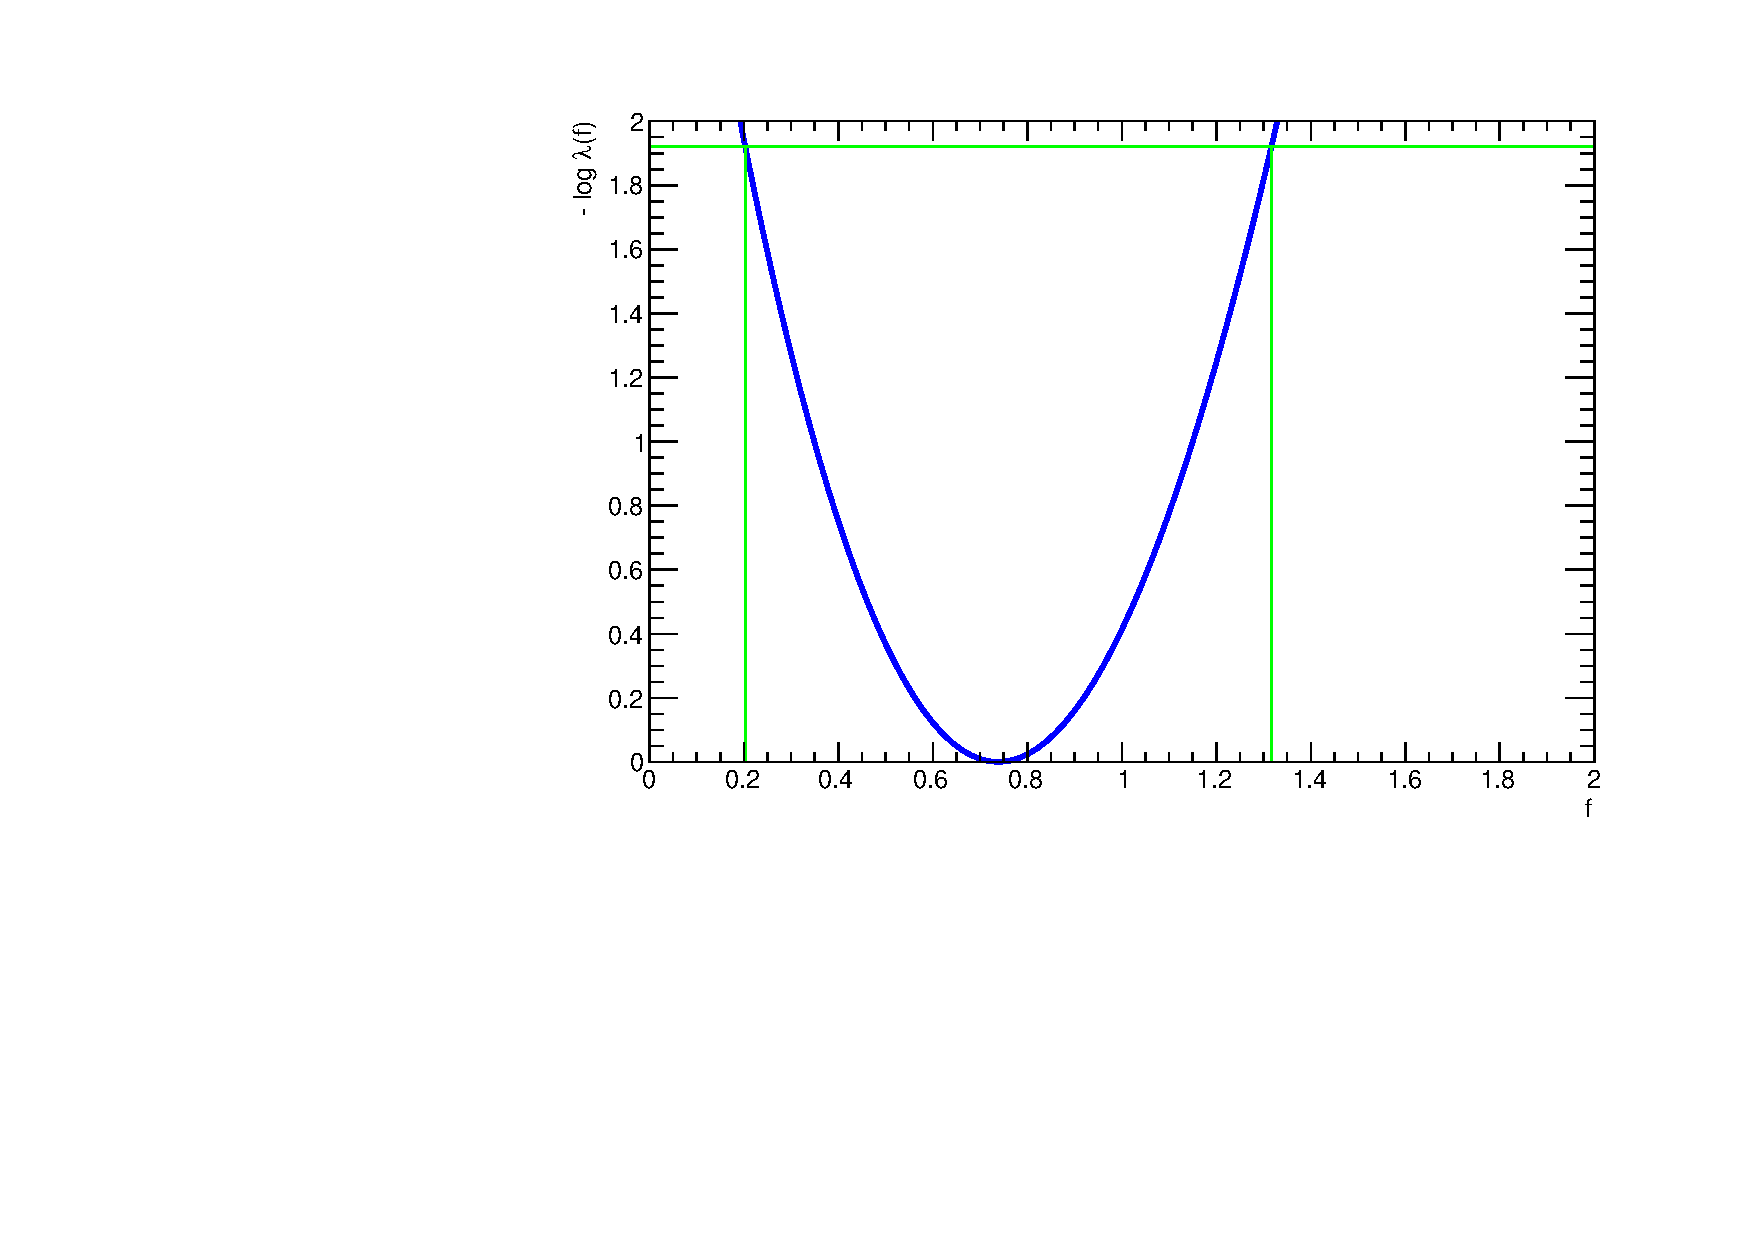
\includegraphics[width=0.45\textwidth]{figures/fit/v22/wSignal/400_100/intervalPlot_2012pf_RQcdZero_fZinvAll_1b_ge4j-1hp_2b_ge4j-1h_signal_95}
    \caption{\label{fig:t2tt-int-400_100}The profile likelihood ratio 
      (defined in Sec.~\ref{sec:cls}) as a function of the signal strength.
      The likelihood considers all data samples under the signal plus SM 
      background hypothesis for the signal model \texttt{T2tt} with 
      $m_{\st} = 400\GeV$ and $m_{\text{LSP}} = 100\GeV$.
      The minimum defines the signal strength estimate which maximizes the
      likelihood and the green vertical line on the right of the minimum 
      indicates the upper-limit at 95\% confidence level.}
  \end{center}
\end{figure*}
\FloatBarrier

\subsection{Comparison with calorimeter jets}

\begin{figure*}[h!]
  \begin{center}
      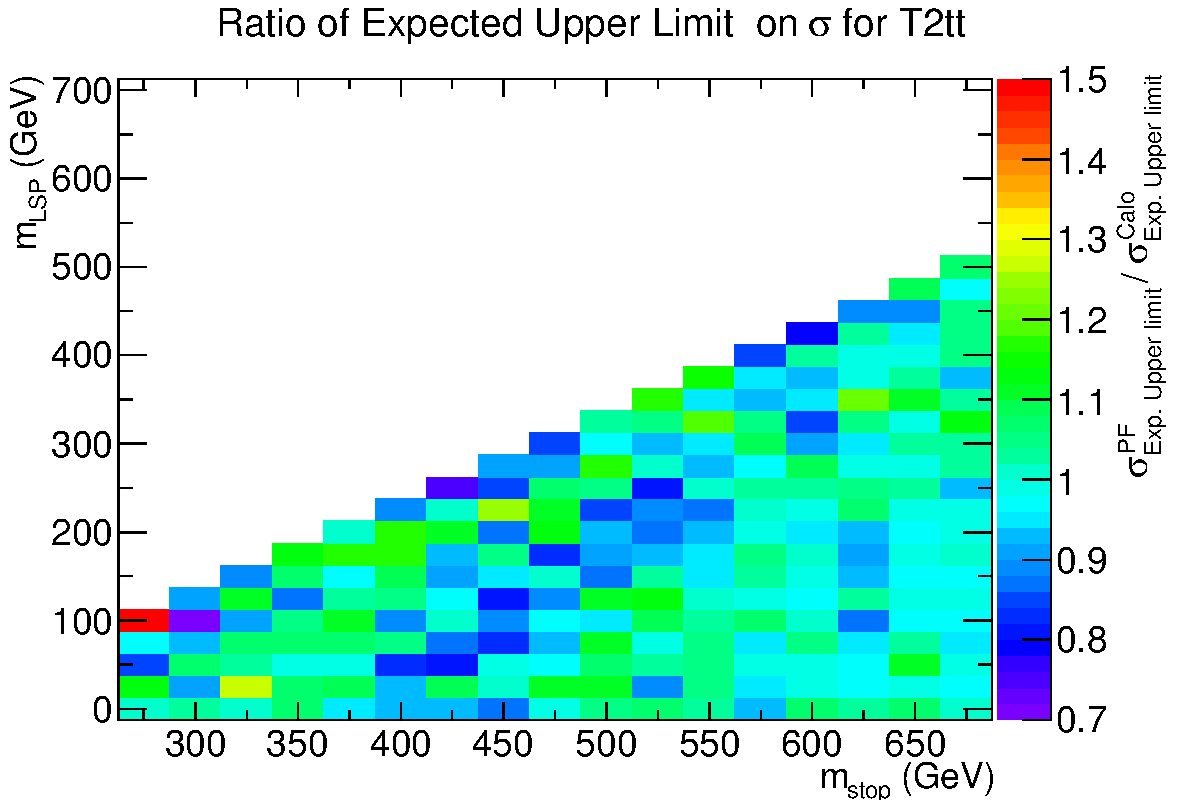
\includegraphics[width=0.65\textwidth]{figures/T2tt_ExpectedUpperLimit_ratio}
    \caption{\label{fig:pfVsCalo}
}
  \end{center}
\end{figure*}

PF-jets have become the predominent jet type used in CMS analyses due to their 
improved reconstruction performence (as discussed in Section~\ref{sec:eventReco}). 
Until now, searches employing the $\alphat$ variable have continued to use calo-jets 
under the assumption that the $\alphat$-triggers (which use calo-jets) would 
introduce too much ineffeciency if any other jet types were used in the offline analysis. 
As this analysis is the first to employ PF-jets with the $\alphat$ variable to search
for excess in all-hadronic events with $\met$ signatures, a comparison with a similar 
calo-jet based analysis is sought. The CMS results using the full 2012 data based on 
calo-jets with have yet to be published, therefore, the comparison is made with 
the analysis described above using calo-jets. The metric for comparison is chosen to 
be the expected upper limit at 95\% C.L. on the cross section of the signal model \text{T2tt} 
as it, by construction, incorporates the efficiency on the signal yields, the background systematic 
uncertainties, and trigger efficiencies. For a given model, the expected upper limit is generally 
considered as the power or sensitivity of a search. Figure~\ref{fig:pfVsCalo} shows the ratio
of expected upper limit at 95\% C.L. between PF-jets and calo-jets, i.e. 
$\frac{\sigma_{\texttt{Exp. Upper limit}}^{PF}}{\sigma_{\texttt{Exp. Upper limit}}^{Calo}}$.
Ratio values $<1$ indicate stronger upper limits set using PF-jets while ratios $>1$ indicate
stronger upper limits set by the use of calo-jets. Throughout the mass plane, the ratios fluctuate
around 1, indicating that altough the $\alphat$ triggers introduce inefficienty (at the order of ~10\% 
in the lowest $\scalht$ bins) when using PF-jets, the jet's reconstruction performance mitigates 
this effect and comparable expected upper limits are achieved. Since PF-jets are now widely used by analyses
and supported by various object performance groups in CMS, any future analysis using $\alphat$ may do
so without concern of loss in sensitivity.  


\FloatBarrier

\subsection{Conclusions}


Years of effort from thousands of people around the world
has brought the LHC and CMS past trough the phases of design, construction,
and commission, to a successful physics run in 2012. CMS recorded more than 
20$\fbinv$ of data and in the process confirmed of the existence of the Higgs boson. 
One of the main motivations to build the LHC still is to conduct
searches beyond the Standard Model; this work presents such a search
in events with jets and missing transverse energy. By using the variable $\alphat$,
the analysis effectively rejects multijet events stemming from QCD and 
mismeasured events. The remaining backgrounds are constrained using
data samples which reduce the reliance on Monte Carlo simulations. Though
a slight excess of observed events over SM prediction is seen in some event categories, 
the observations are found to agree with the expectations of the Standard Model. 
The results are interpreted in two simplified supersymmetric models: (1) a 
pair-produced stop decays into a bottom quark , W boson and neutralino 
(\texttt{T2tt}), (2) a pair-produced stop decays into a charm quark 
jet and a neutralino (\texttt{T2cc}). 
Exclusion limits are set at $m_{\st}>275\GeV$ for $m_{LSP}\sim\!250\GeV$ 
in \texttt{T2cc} and $m_{\st}>400\GeV$ for $m_{LSP}\sim\!50\GeV$ in \texttt{T2tt}. 
The sensitivity achieved in this analysis is similar to that of other 
generic searches in CMS (\cite{CMS-PAS-SUS-14-008,cms-pas-sus-09001})
and ATLAS. The observed limits for \texttt{T2cc} are also comparable 
if not better to other analyses, however the \text{T2tt} exclusion is 
weaker than expected. The LHC will resume operation in the Spring of 
2015 at the center-of-mass energy of 13~\TeV, the \alphat 
analysis as described here will be used to search for signatures of 
pair-production of $\st$, $\sq$ and $\gl$ at this new energy regime.
